%!TEX root = ../Main.tex

\chapter{Vulkan API Overview}
\label{cha:VulkanOverview}
  This chapter provides an overview of the Vulkan \gls{api} and explains some concepts in greater detail.
  It does not cover the entire feature set of Vulkan.
  Most of the information provided in this chapter is based on the Vulkan 1.0 specification~\cite{vkspec}.

  The Vulkan \gls{api}, at its core, is agnostic of the operating system it runs on.
  However, an interface for extending Vulkan is provided that can be leveraged to provide additional functionality to perform platform specific tasks. This is explained in more detail later in this chapter as well as in chapter~\ref{cha:EnvSetup}.

  There are certain terms used throughout this document that refer to specific things in the context of Vulkan development.
  The application that interacts with Vulkan, for instance, is commonly referred to as the \textit{host} or the \textit{host-application}.
  The term \textit{device} refers to the \gls{gpu} and is represented in Vulkan by an object of the same name, which is explained later in this chapter.
  The term \textit{\gls{driver}} refers to the implementation of the Vulkan \gls{api} the application interacts with and is responsible for executing Vulkan \gls{api} commands.
  This is not necessarily the hardware driver itself but is often provided by \glspl{ihv}.

  Throughout this chapter, abbreviated forms are used to refer to several Vulkan commands at once.
  For example, \lstinline{vkPlaceholder*} would refer to all Vulkan commands that begin with the character string \textit{vkPlaceholder}, e.g. \lstinline{vkPlaceholderCommand}. The asterisk is used as a wildcard character.

  \section{Workflow and Patterns}
  \label{sec:WorkflowAndPatterns}
    The Vulkan API was designed to be consistent and explicit.
    Many patterns can be found in the Vulkan code style that make it easier for the \gls{application} to use the API effectively.
    This section is a walkthrough of the basic steps needed to set up a Vulkan graphics pipeline to present an image on a display.

    The first object that has to be created is a Vulkan instance.
    Vulkan makes use of \textit{handle} types allowing the \gls{application} to track objects created with the API.
    The Vulkan instance is represented by such a handle and can be used to query available physical \glspl{device} that provide Vulkan support.
    These physical \glspl{device} can be queried for certain capabilities, such as supported image formats and hardware features, to aid in deciding which physical device to use for the \gls{application}.
    A physical device can subsequently be used to create a logical device, or just device.
    The number of \glspl{device} created from a physical device is not limited by Vulkan but typical applications create just a single instance.
    Devices represent the primary interface to Vulkan and are used for a number of tasks such as allocating \gls{gpu} resources.

    A device also consists of multiple queues which are used to submit work to the \gls{gpu}.
    Queues are logical instances of what is called a queue family.
    Each queue family has certain properties that have to be considered by the application.
    For example, if the queue is supposed to accept submissions of rendering commands, the application needs to ensure the queue actually has graphics capabilities.

    % Queues are created when the associated device is created and are available for as long as the device is available.
    % A device may be associated with multiple queues at once.
    % % This is why there is no \lstinline{vkCreateQueue} but rather \lstinline{vkGetQueue} command.
    % Among other things, \glspl{device} are used to allocate Vulkan objects or GPU memory.
    % Changes made on Vulkan objects do not have global side-effect observable with the regular Vulkan API\todo{Elaborate.
    % Contrast with OpenGL}.
    % However, \glspl{driver} and Vulkan layers or extensions are free to modify their own state across Vulkan object boundaries.\todo{Redundant sentence? This should be a given.}

    Once a device handle has been acquired, the \gls{application} can create a swapchain to establish a connection between a specific queue on the device and a platform specific presentation engine.
    A swapchain contains a number of \textit{presentation images}.
    Usually, these images are used to store the results of the graphics pipelines.
    At the time these images are presented, they have to be in a specific layout reserved for presentation purposes.
    In order for the images to be accepted by the presentation engine, they have to be in a specific layout reserved for presentation purposes.

    In order to render images, a graphics pipeline needs to be created.
    An overview of how graphics pipelines work in general was presented in section~\ref{sec:GraphicsWorkflow}.
    Rendered images produced with a graphics pipeline are then consumed by the presentation engine via a swapchain.
    In Vulkan, a graphics pipeline consists of multiple configurations for fixed-function stages and shader stages.

    Vulkan also provides the concept of a render pass.
    A render pass consists of a list of render targets, called \textit{attachments}, as well as several subpasses that reference the attachments.
    A render pass also stores dependencies between subpasses, that are executed in a specific order, which can be used for post-processing, for example.

    Render passes can be instantiated which is necessary to perform rendering commands.
    Inside a render pass instance, command buffers are used to record rendering commands such as issuing drawing commands or transforming images from one layout to another.
    Command buffers have certain state they can be in which is further explained in section~\ref{sec:CommandBuffers} and chapter~\ref{cha:RenderPipeline}.

    Vulkan objects can be created using \lstinline{vkCreate*} commands with the help of \lstinline{Vk*CreateInfo} structures.
    These info structures contain parameters to create the requested type of object.
    The contents of such info structures are specific to each creation command and require the \gls{application} developer to consult the Vulkan specification in order to provide correct input data.
    All \lstinline{vkCreate*} commands return handles to the objects they create.
    When the object is no longer in use, these handles can be used to destroy the object with the help of \lstinline{vkDestroy*} commands.
    For every \lstinline{vkCreate*} command Vulkan provides a corresponding \lstinline{vkDestroy*} command.
    The commands \lstinline{vkCreateBuffer} and \lstinline{vkDestroyBuffer} are examples for this.

    \todo{Explain memory pools briefly.}When Vulkan objects are allocated from memory pools, or directly from \gls{device} memory, calls to \lstinline{vkAllocate*} commands have to be made.
    These commands are accompanied by \lstinline{vkFree*} commands that return resources to their origin where they originally were acquired from.
    The general rule is that all objects allocated from pools are released as soon as the pool itself is released.
    Using released Vulkan objects results in undefined behavior, similar to using freed memory in \gls{ccpp}.

    Unlike other APIs, Vulkan does not do any object tracking or reference counting to manage object life times.
    It is the responsibility of the \gls{application} to destroy or free Vulkan objects at the appropriate times, i.e.
    when they are no longer in use and will not be used in the future by either the \gls{host} or the device.

    Vulkan objects are generally not designed to be thread-safe.
    The Vulkan specification states whether \gls{host} synchronization is required for each individual command of the \gls{api}.
    This means that accessing or modifying most Vulkan objects from more than one thread at once can lead to race conditions or other undesirable behavior.
    In these cases, it is the responsibility of the \gls{application} to employ proper synchronization mechanisms on the \gls{host} to ensure Vulkan objects are never read from or written to concurrently.

  \section{Layers and Extensions}
  \label{sec:LayersAndExtensions}
    Vulkan is extensible by third-party \glspl{application}.
    The two mechanisms provided are called \textit{layers} and \textit{extensions}.

    A layer in Vulkan can be thought of as an observer to the API calls done by the \gls{application}.
    It does not add new types or commands the \gls{application} can use directly.
    Layers are not required for Vulkan to function properly, they add to and observe existing functionality instead.

    The LunarG SDK~\cite{lunargvulkansdk}, for example, comes with a set of layers to validate usage of the Vulkan API. This is extremely useful during development as it allows application developers to focus on their code rather than the perfect use of the Vulkan API. It should also be noted that bare Vulkan, without any validation layers enabled, does not do any error checking. When the \gls{application} passes an invalid combination of flags to some Vulkan function, it results in undefined behavior and has to be corrected by the \gls{application}.

    As opposed to layers, extensions are able to provide new or add to existing functionality. The motivation for extensions is to keep the Vulkan core functionality small and provide specific functionality via such extensions. In fact, the Khronos Group provides built-in extensions for both common and platform specific functionality.

    \begin{figure}
      \centering
      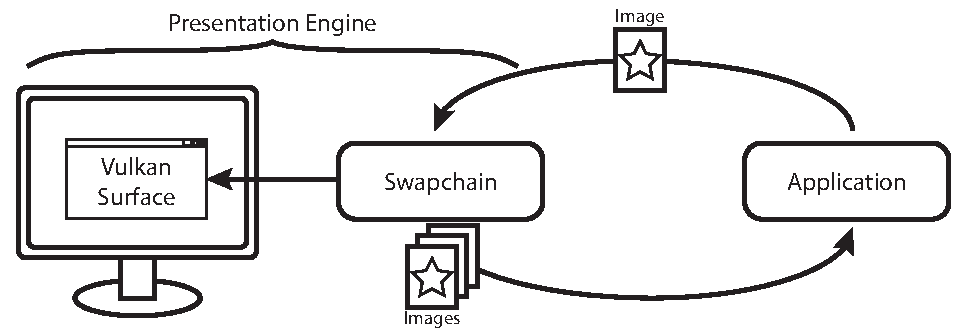
\includegraphics[width=\textwidth]{Main/Images/PresentationEngine}
      \caption{Illustration of the presentation engine being connected to a device using a swapchain.}
      \label{fig:PresentationEngine}
    \end{figure}

    The most important extensions are arguably the swapchain and platform specific surface extensions.
    These extensions enable the \gls{application} to create a Vulkan swapchain and a compatible surface object that is used by the presentation engine to present an image.
    This process is outlined in figure~\ref{fig:PresentationEngine}.
    Vulkan requires the \gls{application} to create a platform specific window which is then used when creating a Vulkan surface.
    This surface is subsequently used to create the swapchain that acts as the connection between a device and the surface.
    With this constellation, the presentation engine is able to properly present an image on a platform specific window.
    The extension to create a swapchain is called
    \lstinline{VK_KHR_swapchain}\footnote{\lstinline{KHR} is short for Khronos and is commonly used to denote extensions developed by the \gls{khronos}.}.
    It adds several types and commands to create and interact with a swapchain.
    The concept of a swapchain is independent of the platform but it requires the help of platform specific functionality in order to work.
    On Windows platforms, for example, the \gls{application} needs to enable the \lstinline{VK_KHR_win32_surface} extension in order to link a swapchain to a Win32 window.
    From the perspective of the \gls{application}, there is no need to care about distinguishing between platforms when creating a swapchain but they do have to when creating and connecting the swapchain to a platform specific surface.

    Extensions can be loaded and enabled on both instance-level and device-level.
    Instance-level extensions are generally independent of the hardware while device-level extensions are usually specific to the individual device.
    The extension \lstinline{VK_EXT_debug_report}, for example, is an instance-level extension.
    It enables the \gls{application} to provide a callback function that is used by Vulkan layers or extensions to communicate with the \gls{application}.
    If validation layers are enabled, this is how they report validation violations to the \gls{application}.
    An example for a device-level extension is the aforementioned \lstinline{VK_KHR_swapchain} extension.
    Not all physical \glspl{device} have to be capable of rendering graphics images.
    In the end it is up to the extension author on which level they provide their extension.

  \section{Resources and Memory Allocation}
  \label{sec:MemoryManagement}
    Memory in Vulkan is categorized in either \gls{host} memory or \gls{device} memory.

    Host memory is used by the \gls{driver} for data structures that are represented by Vulkan objects defined as part of the Vulkan \gls{api}.
    Applications have the option to supply memory allocators to \glspl{driver} in order to control how \gls{host} memory is allocated.
    Host memory allocations are not conducted in performance critical code paths.
    In general, supplying custom memory allocators may not significantly affect efficiency of the \gls{application}.
    Instead, it is an opportunity for \glspl{host} on embedded systems to control memory allocations or for informational purposes such as logging memory allocations done by the \gls{driver}.
    Especially on gaming consoles, where memory typically is a scarce resource, this kind of control will be beneficial to applications.

    The physical storage of a device is called device memory. Device memory is separated into different types of heaps. Each of these heaps has a defined size and a combination of flags. The flags indicate whether memory from that heap is visible to the \gls{host} or whether the memory is completely local to the device. In order for the allocated memory to be useful, the \gls{application} has to bind it to a resource.

    There are two fundamental types of resources in Vulkan, the buffer resource and the image resource.

    \begin{description}
      \item[Buffers]
        A buffer is treated as a one-dimensional, unformatted, contiguous block of memory that can be used by the \gls{application} to upload general purpose data to the device. This data may then be used during shader execution, for example, or may be copied and transformed on the GPU to another buffer or even an image.

        In some circumstances, Vulkan requires a \textit{buffer view} instead of the buffer itself.
        The buffer view contains information about the range and exact layout of formatted data contained in the buffer.
        Multiple buffer views can be used to refer to the same buffer.

      \item[Images]
        As opposed to buffer resources, an image contains more information about how the underlying memory is used. For example, an image has a particular format, such as having red-green-blue channels, each channel using 8 bits of memory. An image may also be in a particular layout, e.g. in \textit{shader read-only} layout which is required when the image is supposed to be used by a shader. Another important image property is the image tiling. An image may either exist in linear tiling or optimal tiling. Linear tiling means that the underlying data of the image is laid out in memory in a linear fashion. The data will be in the same memory layout as it was when it was uploaded. The memory layout of the image data in optimal tiling, however, is not specified by Vulkan. The \gls{driver} is free to lay out the data in memory as it sees fit. This is done in order to improve performance. Parts of the actual physical device may process an image faster in certain circumstances when the image data is not laid out linearly in memory. In addition, special purpose hardware components, such as image samplers, only work in image and not on buffer objects.

        Similar to buffers, images can be referenced via \textit{image views}.
        They contain information about the underlying image, such as the region that is referred to or whether the image is to be interpreted as a 2D image or a cube map.
        This allows applications to use a single image, break it up into several parts covered by image views, and use these parts to perform operations.
        Framebuffers, for example, require image views to be supplied as render targets.
    \end{description}


  \section{Command Buffers}
  \label{sec:CommandBuffers}
    All rendering in Vulkan is done with command buffers.
    Command buffers are allocated from command pools.
    These command pools are managing the memory that is used by all command buffers created from that pool.
    As the name suggests, a command buffer is a container for \gls{gpu} commands.
    Vulkan does not impose any limit on the number or size of commands stored within a single command buffer.

    Command buffers are always in one of three states.
    When a command buffer is created, it is in the \textit{initial} state.
    From this state, the command buffer may transition to the \textit{recording} state by calling \lstinline{vkBeginCommandBuffer}.
    In the \textit{recording} state, as the name suggests, a command buffer is able to record commands using \lstinline{vkCmd*} Vulkan API calls.
    Once all desired commands have been recorded, calling \lstinline{vkEndCommandBuffer} brings the command buffer to the \textit{executable} state.
    In \textit{executable} state, the command buffer may be submitted to a device queue in order to be executed on the \gls{gpu}.
    When submitting a command buffer to the device, it may not be modified until it has finished execution.
    Submitted command buffers will stay \textit{executable} until reset and may even be submitted multiple times.
    In other words, command buffers may be pre-recorded once but submitted multiple times.
    This is particularly useful for rendering static geometry, for example.

    A command buffer may be brought back to the \textit{initial} state by resetting the parent command pool using \lstinline{vkResetCommandPool}.
    Command buffers may be reset individually by calling \lstinline{vkResetCommandBuffer} without the need to reset the entire pool, if the \lstinline{RESET_COMMAND_BUFFER}\footnote{Full name: \lstinline{VK_COMMAND_POOL_CREATE_RESET_COMMAND_BUFFER_BIT}} flag has been set on that pool.
    % If the \lstinline{RESET_COMMAND_BUFFER}\footnote{Full name: \lstinline{VK_COMMAND_POOL_CREATE_RESET_COMMAND_BUFFER_BIT}} flag has been set on the pool, an \textit{executable} command buffer may be individually reset by calling \lstinline{vkResetCommandBuffer} without the need to reset the entire pool.
    In addition, with that flag present, a command buffer may even be brought to the \textit{recording} state directly by simply calling \lstinline{vkBeginCommandBuffer} again, discarding all internally buffered commands up to that point.

    There are two types of command buffers called \textit{primary} and \textit{secondary} command buffers.
    Primary command buffers may be submitted to device queues and are able to execute secondary command buffers.
    Secondary command buffers can not be submitted directly to device queues, they can only be executed by primary command buffers.
    Secondary command buffers are also unable to execute other command buffers.

  \section{Render Passes}
  \label{sec:RenderPassesOverview}
    Vulkan defines the concept of \textit{render passes} that describe the kinds of data that are involved when rendering is performed on the \gls{gpu}.
    It consists of multiple subpasses, descriptions of dependencies between these subpasses, as well as a specification of all targets, called \textit{attachments}, that are involved in the rendering process. Figure~\ref{fig:RenderPassOverview} provides an overview how subpasses are referencing the attachments in the render pass, each requiring the referenced attachment to be in different kinds of formats.

    \begin{figure}
      \centering
      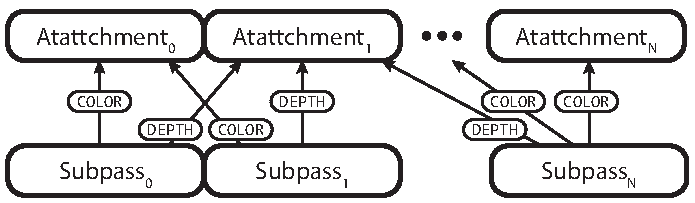
\includegraphics[width=\textwidth]{Main/Images/RenderPassOverview}
      \caption{Overview of a render pass that consists of multiple attachments and subpasses that reference these attachments.}
      \label{fig:RenderPassOverview}
    \end{figure}

    A render pass is required when recording commands to a command buffer.
    At some point during command buffer recording, the application calls \lstinline{vkBeginRenderPass} which creates an \textit{instance} of the render pass.
    This instance stores several other information, such as clearing values, the framebuffer used for rendering, the area on the framebuffer to render to, and more.
    Command buffer recording is performed on a per-subpass basis, hence each render pass needs at least one subpass, otherwise it would not be possible to record rendering commands.

    Subpasses provide a way to connect different pipelines, which are presented in the next section, in such a way that the output of one subpass may be used as input by another subpass.
    This can be useful for post-processing, for example.
    However, in many circumstances, a single subpass is sufficient.

  \section{Pipelines}
  \label{sec:Pipelines}
    % \todo[inline]
    % {
    %   Describe descriptor-sets, descriptor-pools, etc?

    %   Explain "Binding Points" somewhere.
    % }

    \begin{figure}
    % \begin{wrapfigure}{r}{0.45\textwidth}
      \label{fig:GraphicsPipeline}
      \centering
      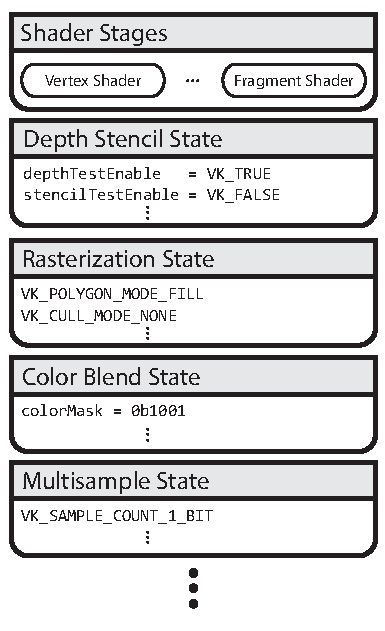
\includegraphics[height=0.4\textheight]{Main/Images/GraphicsPipeline}
      \caption{Incomplete list of graphics pipeline components and examples of their individual properties.}
    % \end{wrapfigure}
    \end{figure}

    Vulkan uses the concept of pipelines to describe how work is performed on the GPU.
    It supports compute and graphics pipelines.
    The compute pipeline consists only of a single programmable stage.
    The graphics pipeline, however, is considerably more complex.
    It has multiple fixed-function stages and five programmable stages, called shader stages.
    Some of the fixed-function stages have configurable state that can be manipulated by the \gls{application}.
    For example, the rasterization stage can be configured to interpret incoming vertex data as either a list of points, lines, or filled polygons with more than two sides.
    Figure~\ref{fig:GraphicsPipeline} provides an overview of some of the components of the graphics pipeline.

    Programs that are designed for use in shader stages are called shaders.
    Shaders are supplied to Vulkan in \gls{spirv} format.
    \gls{spirv} is a high-level graphics and parallel compute programming language provided in binary form.
    The specification of \gls{spirv} is entirely maintained by the the Khronos Group~\cite{spirvspecprov}.
    More information about \gls{spirv} is provided in chapter~\ref{cha:EnvSetup}.

    When defining a graphics pipeline, Vulkan requires the \gls{application} to at least specify a vertex shader.
    All other shader stages are optional.
    A graphics pipeline also has a specific layout that is specified in terms of the vertex input layout and the descriptor set layout.
    The vertex input layout describes how the data in vertex buffers is to be interpreted.
    The descriptor set layout describes the kind of data that is used by shaders, like uniform buffers or image samplers.

    % \todo[inline]{Describe why having only a vertex shader stage can be useful? (Cache skinning results)}

    \begin{figure}
      \label{fig:RenderPassInstanceSample}
      \centering
      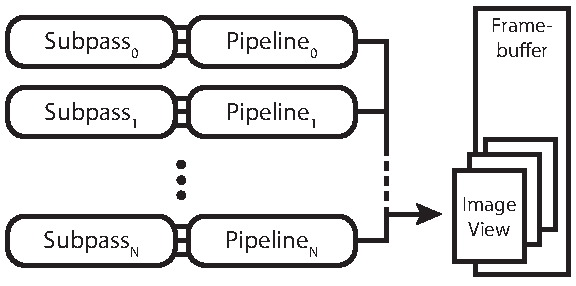
\includegraphics[width=\textwidth]{Main/Images/RenderPassInstanceSample}
      \caption{Overview of a render pass instance with a framebuffer and bound pipelines.}
    \end{figure}

    Pipelines are tightly connected to render passes.
    In fact, when creating a pipeline, the index of the subpass the pipeline will be executed in has to be known already.
    Render pass objects, as explained earlier in section~\ref{sec:RenderPassesOverview}, contain information about the dependencies between pipelines as well as information about the framebuffer attachments.
    But pipelines are interchangeable and do not store information about other pipelines that are executed before or after them.
    % Creating a connection between pipelines in the render pass allows the \gls{driver} to perform optimizations.
    Figure~\ref{fig:RenderPassInstanceSample} shows how each pipeline is connected to a render pass to produce results stored in a connected framebuffer.

    \subsection{Pipeline Cache}
    \label{subsec:PipelineCache}
      Creating pipeline objects is a fairly heavyweight operation.
      To speed up pipeline creation, Vulkan provides what is called a pipeline cache.
      When creating a pipeline, such a pipeline cache object can be supplied by the \gls{application}.
      Vulkan will try to find a matching pipeline in the cache.
      If it finds a matching pipeline, it is loaded from the cache instead of creating a new one.
      If no such pipeline is found in the pipeline cache, a new pipeline is created and written to the pipeline cache.
      Vulkan provides a command to retrieve the serialized pipeline cache, which can be saved by the \gls{application} in whatever location is most convenient to it.
      This serialized pipeline cache can then be fed back to Vulkan at a later time.

      Pipeline cache objects are managed by the \gls{driver} and are internally synchronized.
      This means that a single pipeline cache object can be used throughout the entire application without having to worry about synchronization in multi-threaded contexts.


  \section{Synchronization}
    Vulkan was designed to scale well in multi-threaded environments.
    However, most \gls{api} call synchronization has to be performed by the application.
    The application typically knows best when synchronization is needed, if any is needed at all, which is why this approach is employed in the Vulkan \gls{api}.

    Vulkan does not provide synchronization primitives that can be used exclusively on the \gls{cpu}.
    However, Vulkan provides synchronization primitives for inter-\gls{gpu} and \gls{cpu}--\gls{gpu} synchronization.
    These synchronization primitives are fences, semaphores, events, and barriers which are explained in the following sections.

    \subsection{Fences}
    \label{sub:Fences}
      A fence is a synchronization primitive used to determine the execution status of submitted operations executed in a queue.
      Such a fence can only be in one of two states: not signaled and signaled.
      The status of a fence is visible to the \gls{host}.
      The device itself does not use the status of a fence directly.

      The most common way a fence is used is when submitting work to a queue via the \lstinline{vkQueueSubmit} command.
      The supplied fence is signaled once all work in that submission has been completed.
      The \gls{application} can query the submitted fence for its status using \lstinline{vkFenceGetStatus} to determine whether the fence was signaled yet or not.
      Waiting for a fence to be signaled essentially means waiting for all of the submitted work on the queue to be finished.
      Using the \lstinline{vkWaitForFences} \gls{api}, the application can wait for one or more fences to be reached, halting execution of the application on the \gls{cpu} for that time.

    \subsection{Semaphores}
    \label{sub:Semaphores}
      A semaphore is similar to a fence, as discussed above in~\ref{sub:Fences}, except that its status is only visible to the device.
      It can be used to synchronize operations within the same and between different device queues.

      The most common use case for Vulkan semaphores in a graphics \gls{application} is when presenting swapchain images to the presentation engine.
      First, the commands to create the final image have to be recorded to a command buffer.
      This command buffer then needs to be submitted to a queue in order to be executed.
      When submitting to the queue, a semaphore can be provided that will be signaled once the queue has finished executing all submitted commands.
      The same semaphore can be used when issuing the swapchain presentation command.
      When everything is set up like this, the presentation engine will effectively wait for the commands to produce the final image and then present it immediately.

      % Note that a fence can be used to achieve the same results except that it would require the \gls{host} to actively wait for the queue to finish executing, stalling any other CPU operations that could have been executed in that time.
      Note that a fence can be used to achieve the same results.
      However, a fence would require the \gls{host} to actively wait for the queue to finish executing, reducing processing time that could be spent on other computations.
      Using a semaphore will result in better performance in this case.

    \subsection{Events}
    \label{sub:Events}
      \todo[inline,color=blue!60]{Investigate: Event host-callbacks? Or does the host need to poll?}

      Events are used to synchronize between \gls{host} and device or between device and device in a bidirectional manner.
      Like semaphores and fences, events are either in a signaled or in a not-signaled state.
      Events are inserted into command buffers in order to allow the device to signal them.
      This allows for more fine-grained synchronization between commands and to signal command completion to the \gls{host}.
      Unlike a fence, an event can be inserted at any point in the command buffer stream and thus can be used to query for synchronization without requiring that all commands in the submitted command buffer have completed execution.

      Events work in a way that can be taken advantage of when faced with a scenario that requires the \gls{application} to transform a large number of resources in batches.
      Given an arbitrary number of images in an \gls{application} that need to be transformed in some way that is expensive to compute, these transformations could be issued into a single command buffer, inserting a completion event between these commands.
      After submitting this command buffer to the queue, the \gls{application} can periodically query for completion of the individual transformation commands without the need to wait for the entire submission to finish by using fences or semaphores.

      It must be noted that events are only allowed to be inserted into command buffers that are all submitted to the same queue.
      This makes them unsuitable for cross-queue synchronization when such is required.

    \subsection{Barriers}
    \label{sub:Barriers}
      \proofread
      Barriers are used to synchronize \gls{gpu} commands.
      There are two kinds of barriers in Vulkan.
      The first kind is called an execution barrier which is used to create explicit dependencies on the completion of specific commands.
      The second kind is called a memory barrier which is used to set up a dependency for specific resources or regions of memory.

      \begin{figure}
        \centering
        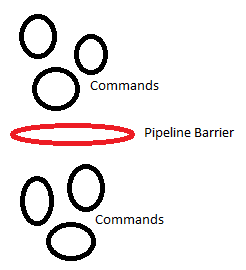
\includegraphics[width=\textwidth]{Main/Images/PipelineBarrier}
        \caption{Illustration of a pipeline barrier inserted between commands in a command buffer.}
        \label{fig:PipelineBarrier}
      \end{figure}

      \proofread
      By inserting a memory dependency using a memory barrier, Vulkan guarantees that all memory operations on a specified resource or memory region have finished once the inserted barrier has been reached, preventing subsequent memory operations from executing until that point.
      Analogously, an execution dependency requires all previous commands to have finished execution before starting to execute other commands inserted after the barrier.
      \proofread
      Figure~\ref{fig:PipelineBarrier} illustrates such a case.

      There are three types of memory barriers in Vulkan: Global memory barriers, buffer memory barriers, and image memory barriers.

      \subsubsection{Global Memory Barriers}
        Global memory barriers introduce a dependency to all memory objects that exist at the time of execution of the barrier.
        All prior memory access operations, whether they are read or write operations, must have finished before the barrier is reached.

        Such heavyweight memory dependencies are not needed if the memory in use is entirely cache coherent.
        In other words, if the rest of the system ensures that all caches are flushed at appropriate times, memory accesses from other parts of the system will be consistent and up-to-date.
        % \todo{Double-Triple-Check whether this is actually correct.}{}

      \subsubsection{Buffer Memory Barriers}
        Buffer memory barriers introduce a memory access dependency on a specific region of memory associated with a buffer object.
        That region may encompass the entire buffer and is specified in terms of an offset, relative to the beginning of the buffer, and a size value.

        This kind of barrier can be used to transfer ownership of a buffer region to another queue family or to change access flags of that region.
        Transferring ownership of that buffer region to another queue family is only possible if this kind of operation has been enabled for that buffer at the time it was created.
        Access flags are used to control how the buffer region is accessed.
        They could be used to make the memory region read-only, for example, or enable \gls{host} access for it.

      \subsubsection{Image Memory Barriers}
        Image memory barriers are similar to buffer memory barriers.
        They can be used to transfer ownership of image regions to another queue family, modify access flags, and change the image layout.
        An image region is specified differently from a buffer region because of the fact that images need not be stored linearly in \gls{device} memory.
        More information about images is provided in section~\ref{sec:MemoryManagement}.

        Transferring ownership of an image region is only possible if the image was set up accordingly at creation time.
        Modifying access flags has the same effect as with modifying access flags on a buffer region.

        Changing the layout of the image is an important operation on Vulkan images.
        For example, it is required for swapchain images in order to be presentable.
        The presentation engine requires swapchain images to be in a specific layout when presenting them so the \gls{application} must ensure that the image has that specific layout before attempting to issue the presentation command.
        Since the presentation layout is only meant for use by the presentation engine, the \gls{application} has to use another image memory barrier to change the layout into something that can be used by the \gls{host} \gls{application}.
